\chapter{Ergebnisse}
\label{ch:results}

In diesem Kapitel werden die Ergebnisse der in \autoref{sec:experimente} beschriebenen Experimente vorgestellt.
Die Evaluation schließt die Ergebnisse aller vier Phasen, häufige Fehler in der Verifikation, sowie eine grobe Kategorisierung der Aktionsklassen ein.

\section{Benchmark}
\label{sec:benchmark}

In diesem Abschnitt werden die Rechenergebnisse der verschiedenen Modelle miteinander verglichen.
Als Baseline-Modelle werden R2+1D-34, ir-CSN-152 und zwei Varianten von SlowFast-50 getestet und dabei mit $\Theta_\text{train} = 200$ für 10 Epochen nachtrainiert.
Beide SlowFast-Varianten wurden zunächst ohne Hinzunahme von Non-Local-Blöcken trainiert.
In \autoref{tab:phase1} sind die Ergebnisse zu sehen, wobei alle Hyperparameter aus den ursprünglichen Publikationen übernommen wurden.
Die Metriken basieren auf einem einheitlichen Testset mit $\Delta_\text{test} = 3$.
Der Zeitkontext im Testset ist damit größer als im Trainingsset und wird durch zusätzliche Frames erreicht (\zB 36 statt 32 Frames bei ir-CSN), die die Modelle durch ihr dynamisches Pooling wieder auf die passende Länge stauchen.

Überraschend ist, dass die SlowFast-Variante mit $\alpha = 8$ (SlowFast-50-4x16) bessere Ergebnisse erzielt als die Variante mit $\alpha = 4$ (SlowFast-50-8x8).
Im ersteren erhält der Slow-Pathway schließlich nur halb so viele Frames, wie im letzteren und kann sich damit noch mehr auf räumliche Features fokussieren.
Da die Ergebnisse für SlowFast-50-4x16 durchweg besser ausfallen, wird diese Variante im weiteren Verlauf als SlowFast-Baseline-Modell bezeichnet.

\begin{table}
    \centering
    \small
    \csvreader[no head,tabular=|l|r||r|r|r|r|,
    table head=\hline,late after line=\\\hline]{tbl/exp_phase_1.csv}
    {1=\model,2=\aurocval,3=\baval,4=\fbetaval,5=\lr,6=\bs,7=\ba,8=\rec,9=\prec,10=\auroc}
    {\model & \lr & \ba & \prec & \rec & \auroc}
    \caption[Ergebnisse aus Benchmark]{Ergebnisse aus Benchmark\footnote{Ergebnisse und Beispiele online unter https://www.comet.ml/narendorf/socc-har-32-benchmark}: Getestet mit $\Delta_\text{test} = 3$}
    \label{tab:phase1}
\end{table}

\subsection{Vergleich der Modelle}
\label{subsec:vergleich-der-modelle}

Vergleicht man die Ergebnisse, fällt auf, dass ir-CSN die besten und R2+1D die schwächsten Metriken vorweist.
Damit einher geht allerdings auch ein größerer Fußabdruck:
während bei R2+1D (\bzw SlowFast) eine maximale Batch-Größe von 24 (\bzw 21) möglich war, erlaubt ir-CSN nur eine Batch-Größe von maximal 5 bei gleicher Speicherauslastung.
Dennoch wird für den weiteren Verlauf ir-CSN als einziges Baseline-Modell weitergeführt.
Die weitere Optimierung der anderen Modelle wird aus Zeitgründen nicht weiter verfolgt.

\subsection{Verifikation}
\label{sec:verifikation}

Im nächsten Schritt werden die Fehler der Experimente genauer analysiert.
Grundlage sind die drei Baseline-Modelle aus der ersten Phase.
Im Zuge der Analyse werden innerhalb einer statistischen Analyse Auffälligkeiten im Fehlerreport analysiert.
Zusätzlich werden jeweils 50 der Samples mit den größten Fehlerwerten innerhalb eines Experiments verifiziert.

Bei der statistischen Analyse werden die Samples nach Halbzeitvideo gruppiert und der Mittelwert der Fehler wird berechnet.
Dadurch konnten insgesamt vier fehlerhafte Videos erkannt werden, da diese auffällig hohe Mittelwerte hatten (mit einem z-Score über 3).
Zudem wurde für zwei weitere Videos, die nach dem gleichen Kriterium aufgefallen sind, das manuelle Aligning nachjustiert.

Bei der Verifikation einzelner Samples wurden pro Modell 50 Samples (im Verhältnis 3:1:1 je Datensubset) mit den höchsten Fehlerwerten manuell verifiziert.
Dies entspricht 150 Samples, bei denen insgesamt 267 Transaktionen mit Korrekturvorschlägen gespeichert wurden.
Die Transaktionen bestehen zu 72.6 \% aus Zeitfensteranpassungen.
22.8 \% sind Löschungen von nicht sichtbaren Aktionen und 4.5 \% sind hinzugefügte Aktionen.
Die häufigsten Klassen für Zeitfensteranpassungen sind \code{save} (32), \code{footShot} (30), \code{cross} (14) und \code{card} (10).
Besonders auffällig ist, dass \zB \code{save}- oder \code{card}-Aktionen in den Stammdaten teils mehrere Sekunden zu früh auftreten.
Nach Durchsicht der Daten werden die 267 Transaktionen in die Datenbank übernommen.
Alle weiteren Experimente beziehen sich somit auf die korrigierte Datenbank.

Eine weitere Optimierung des Baseline-Modells (ir-CSN) mit der verifizierten Datenbank, führt zu einer zusätzlichen Steigerung der Balanced Accuracy von 1.6\% Prozent (siehe \autoref{tab:phase1}).

\section{Hyperparameter-Optimierung}
\label{sec:hyperparameter-optimierung}

Das Baseline-Modell der ersten Phase bildet mit $T=32$ und $\tau = 2$ einen Zeitkontext von $\Delta_\text{fit}=2.67$ Sekunden ab.
Da diese Hyperparameter auf Grundlage eines anderen Datensets festgesetzt wurden, werden die oben genannten Hyperparameter im nachfolgenden Experiment in einer Grid-Suche anhand des vorliegenden Datensets angepasst.
Das Vorgehen ist weiter motiviert durch die Mindestdauer von 4 Sekunden in SoccerDB \bzw der unteren Grenze von 3 Sekunden basierend auf \gls{sbod}.

Alle Modelle nutzen ein dynamisches Avg-\pool-Layer zwischen dem letzten \conv- und dem ersten \fc-Layer, das die Verarbeitung von \glspl{clip} variabler Länge $T$ zulässt.
Um eine geeignete Methode zu finden, wird der Einfluss von Avg-Pooling durch ein höheres $T$ und von schnelleren \glspl{clip} durch einen höheren Zeitschritt $\tau$ verglichen.
Die Grid-Suche betrachtet also Punkte für verschiedene Werte von $T$ und $\tau$, wobei der dadurch beeinflusste Zeitkontext \gls{tld:Delta} sich innerhalb der unteren und oberen Grenze von 3 \bzw 6 Sekunden bewegen soll.
Für die Wahl von $T$ werden sechs Werte zwischen 24 und 64 getestet, wobei 64 die maximale Anzahl von Frames darstellt.
Zusätzliche Frames würden die Kapazität der \gls{gpu} überschreiten und sind im Rahmen dieser Arbeit technisch nicht möglich.
Die Punkte für $\tau$ werden so gewählt, dass sich der resultierende Zeitkontext etwa um eine Sekunde unterscheidet.
Zusätzlich wird das Baseline-Modell der vorherigen Phase erneut getestet.
\autoref{fig:exp-hparams-grid} zeigt alle getesteten Punkte der Grid-Suche, sowie Orientierungslinien für den Zeitkontext.

\begin{figure}
    \centering
    \begin{subfigure}{.25\textwidth}
        \centering
        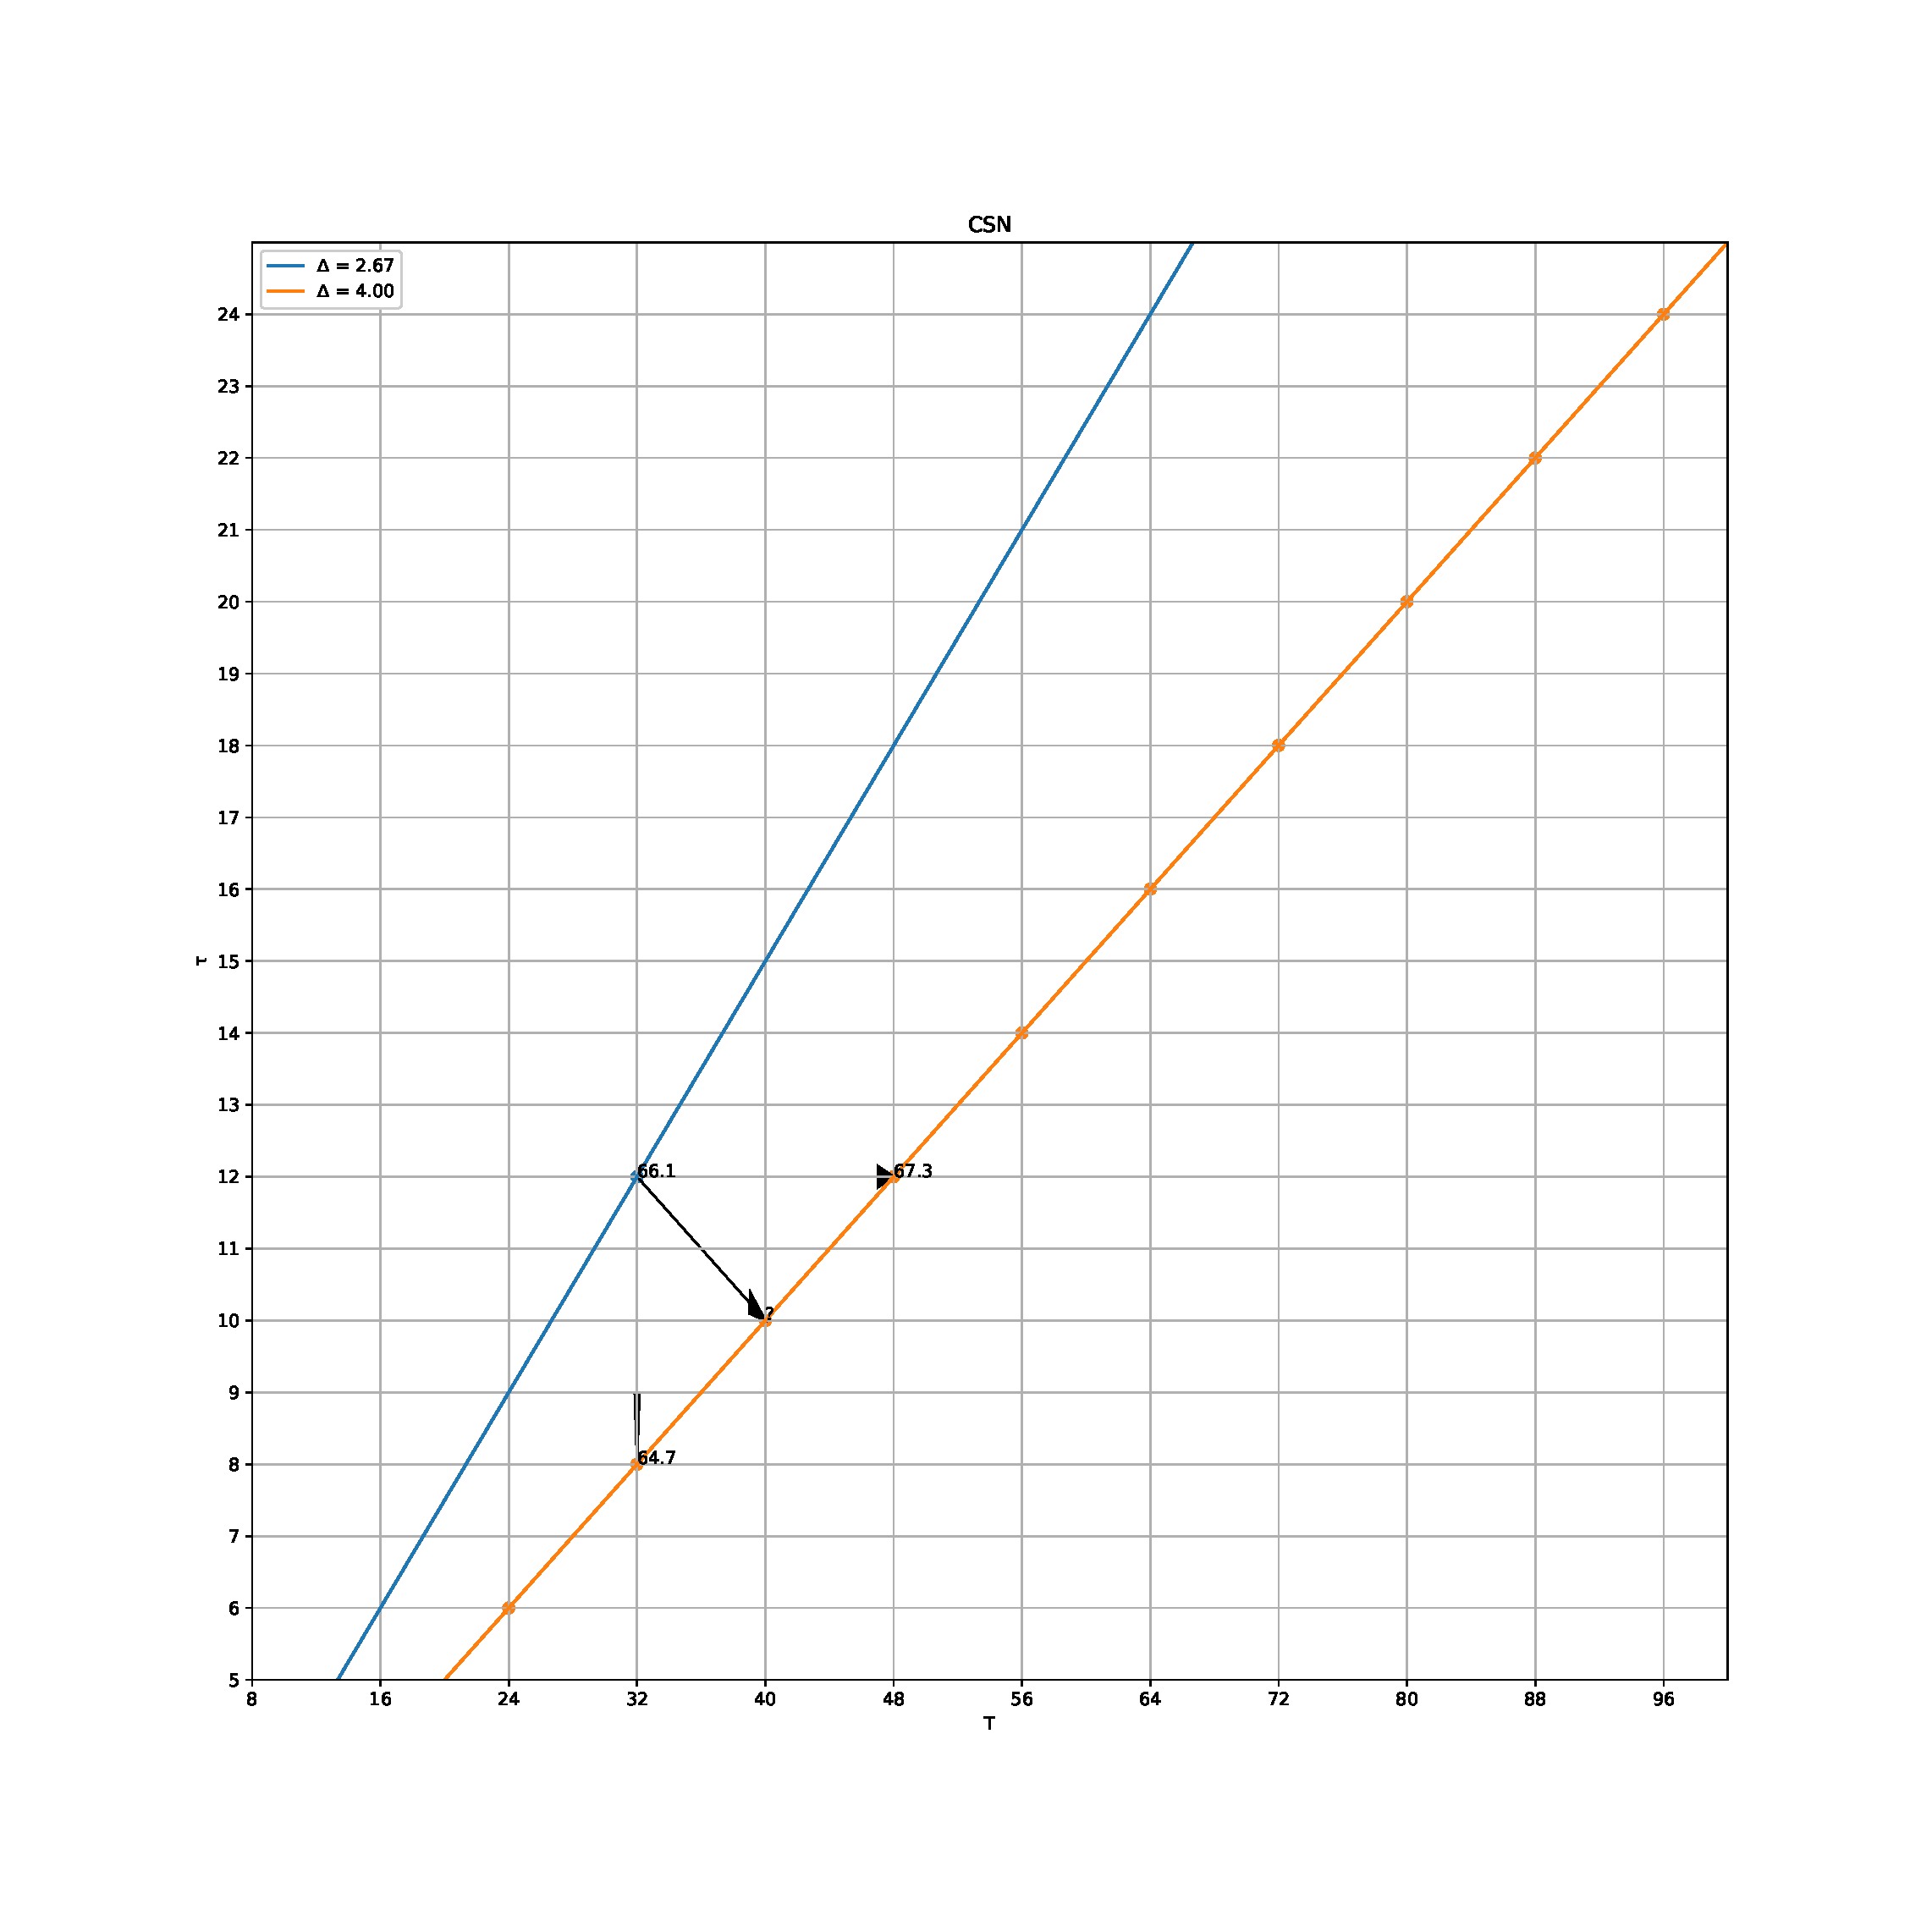
\includegraphics[width=0.99\textwidth, keepaspectratio, interpolate]{img/07_grid_csn.eps}
        \caption{Punkte für Grid-Suche}
        \label{fig:exp-hparams-grid}
    \end{subfigure}%
    \hfill
    \begin{subfigure}{.37\textwidth}
        \centering
        \includegraphics[width=0.99\textwidth, keepaspectratio, interpolate]{img/07_par_cor_prec.eps}
        \caption{Precision für Grid-Suche}
        \label{fig:exp-hparams-prec}
    \end{subfigure}
    \begin{subfigure}{.37\textwidth}
        \centering
        \includegraphics[width=0.99\textwidth, keepaspectratio, interpolate]{img/07_par_cor_rec.eps}
        \caption{Recall für Grid-Suche}
        \label{fig:exp-hparams-rec}
    \end{subfigure}
    \caption[Punkte und Ergebnisse der Grid-Suche zur Hyperparamter-Optimierung]{Punkte und Ergebnisse der Grid-Suche zur Hyperparamter-Optimierung (Quelle: Eigene Darstellung)}
\end{figure}

Aufgrund der Vielzahl zusätzlicher Experimente wird die Laufzeit bei diesen Experimenten durch $\Theta_\text{train} = 100$ und auf 3 Epochen begrenzt.
Da das Baseline-Modell nach der ersten Phase bereits neue Feature gelernt hat, wird zu Beginn eine neue Lernrate gesucht, die für alle Trainings der Grid-Suche gilt und dem Intervall $[3e^{-4}, 3e^{-6}]$ entspricht.
\autoref{fig:exp-hparams-prec} und \autoref{fig:exp-hparams-rec} veranschaulichen die Ergebnisse der Grid-Suche in Form von Parallelen Koordinaten.
Es fällt auf, dass die Hyperparameter sehr gegensätzlichen Einfluss auf die Metriken Precision und Recall haben.
So wirken sich zusätzliche Frames und ein hoher oder gleichbleibender Zeitschritt positiv auf den Recall aus, während sich beides eher negativ auf die Precision auswirkt.
Ein erhöhter Zeitkontext wirkt sich ebenfalls positiv auf den Recall auf.
Die Precision scheint hingegen unabhängig vom Zeitkontext zu sein.

\begin{table}
    \centering
    \small
    \csvreader[no head,tabular=|r|r|r||r|r|r|,
    table head=\hline,late after line=\\\hline]{tbl/exp_phase_2.csv}
    {1=\model,2=\s,3=\t,4=\sr,5=\d,6=\auroc,7=\ba,8=\fone}
    {\t & \sr & \d & \ba & \fone & \auroc}
    \caption[Ergebnisse aus Hyperparameter-Optimierung]{Ergebnisse aus Hyperparameter-Optimierung\footnote{Ergebnisse und Beispiele online unter https://www.comet.ml/narendorf/socc-har-32-grid-search}: ir-CSN-152 getestet mit $\Delta_\text{fit} = 4.8$}
    \label{tab:phase2}
\end{table}

Um ein gutes Gleichgewicht zwischen den beiden Metriken zu erlangen, werden nachfolgend nur noch Ergebnisse betrachtet, die einen besonders hohen F1-Score aufweisen.
In \autoref{tab:phase2} sind nur Experimente gelistet, die maximal 1 \% vom maximalen F1-Score abweichen.
Als zusätzlicher Filter werden Experimente ausgeschlossen, deren Balanced Accuracy mehr als 1 \% vom Maximum abweicht.
Als Baseline-Modell für die nachfolgenden Experimente wird die Konfiguration mit $T=48$ und $\tau=2.4$ (10 \gls{fps}) gewählt.
Da sich für dieses Modell ein Zeitkontext von $\Delta_\text{fit} = 4.8$ ergibt, wird für dieses und alle folgenden Experimente ein zweites Testset gesamplet mit $\Delta_\text{test} = 5$.
Das neue Baseline-Modell wird erneut für 5 Epochen mit $\Theta_\text{train} = 200$ trainiert und liefert dabei eine Balanced Accuracy von 68.18~\% auf dem neuen Testset.

\section{Kategorisierung der Aktionsklassen}
\label{sec:kategorisierung-der-aktionsklassen}

In den bisherigen Experimenten wurden jeweils nur die durchschnittlichen Metriken (macro) über alle Klassen betrachtet.
In diesem Abschnitt wird das Baseline-Modell der zweiten Phase erstmals pro Klasse evaluiert.
Dabei werden besonders schwere Klassen aus dem Datenset entfernt und das Modell wird ohne diese Klassen erneut nachtrainiert.

Zuerst werden die Metriken des vorangegangenen Experiments pro Klasse erhoben.
\autoref{fig:ba_by_class} zeigt die Balanced Accuracy zum Baseline-Modell aus Phase 2.
Dem ist zu entnehmen, dass es teils sehr starke Abweichungen innerhalb der verschiedenen Klassen gibt.
Während Aktionen wie \code{corner}, \code{footShot} oder \code{throwIn} hohe Werte vorweisen, können andere Klassen wie \code{offside} oder \code{handball} fast gar nicht korrekt klassifiziert werden.

%Das wird insbesondere deutlich wenn man die Metriken Precision und Recall in \autoref{fig:precision-recall} betrachtet.

\begin{figure}
    \centering
    \begin{subfigure}{.24\textwidth}
        \centering
        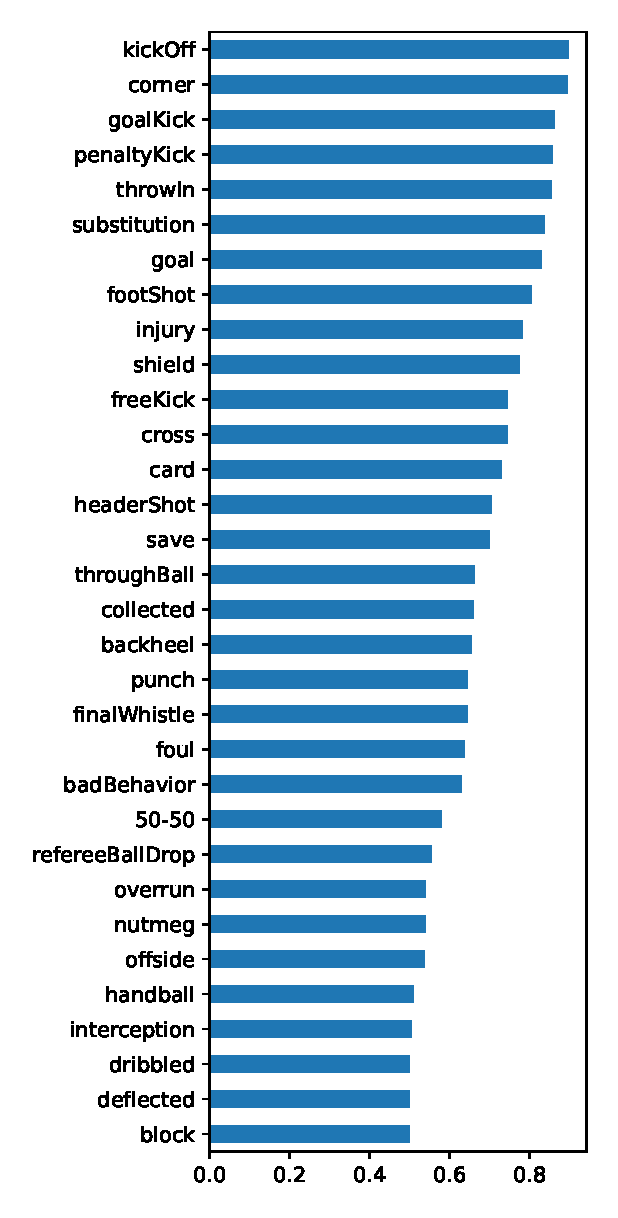
\includegraphics[width=0.99\textwidth, keepaspectratio, interpolate]{img/07_ba_by_class_ph_2.eps}
        \caption{Balanced Accuracy \newline mit 32 Klassen}
        \label{fig:ba_by_class}
    \end{subfigure}%
    \begin{subfigure}{.24\textwidth}
        \centering
        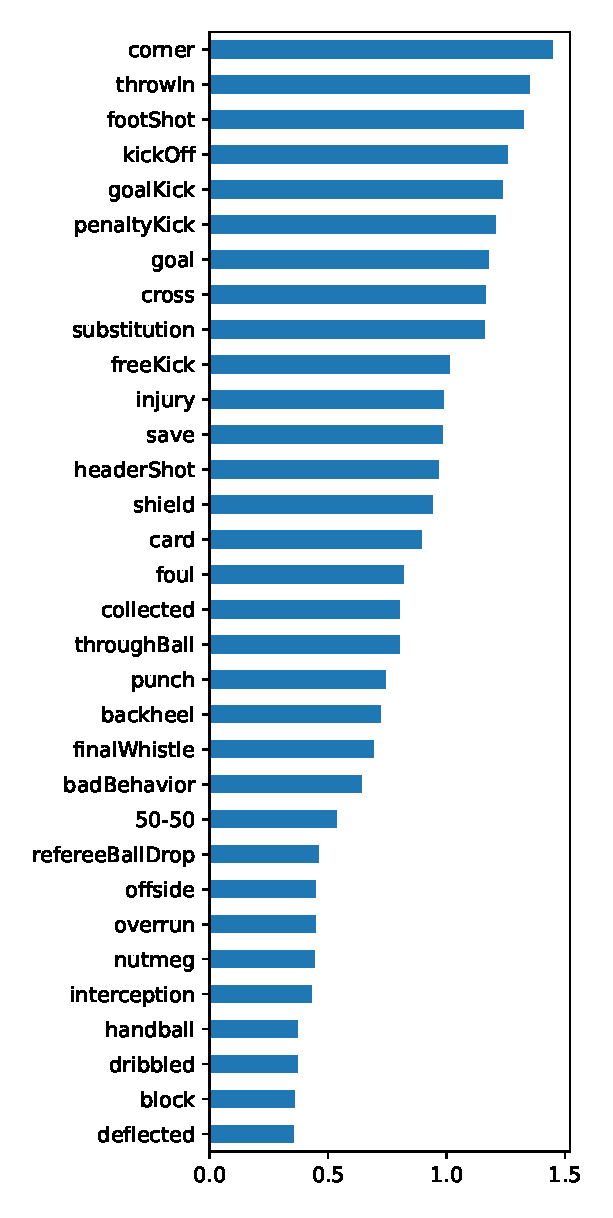
\includegraphics[width=0.99\textwidth, keepaspectratio, interpolate]{img/07_pca_by_class_ph_2.eps}
        \caption{PCA-0 \newline mit 32 Klassen}
        \label{fig:pca_by_class_phase_2}
    \end{subfigure}
    \begin{subfigure}{.24\textwidth}
        \centering
        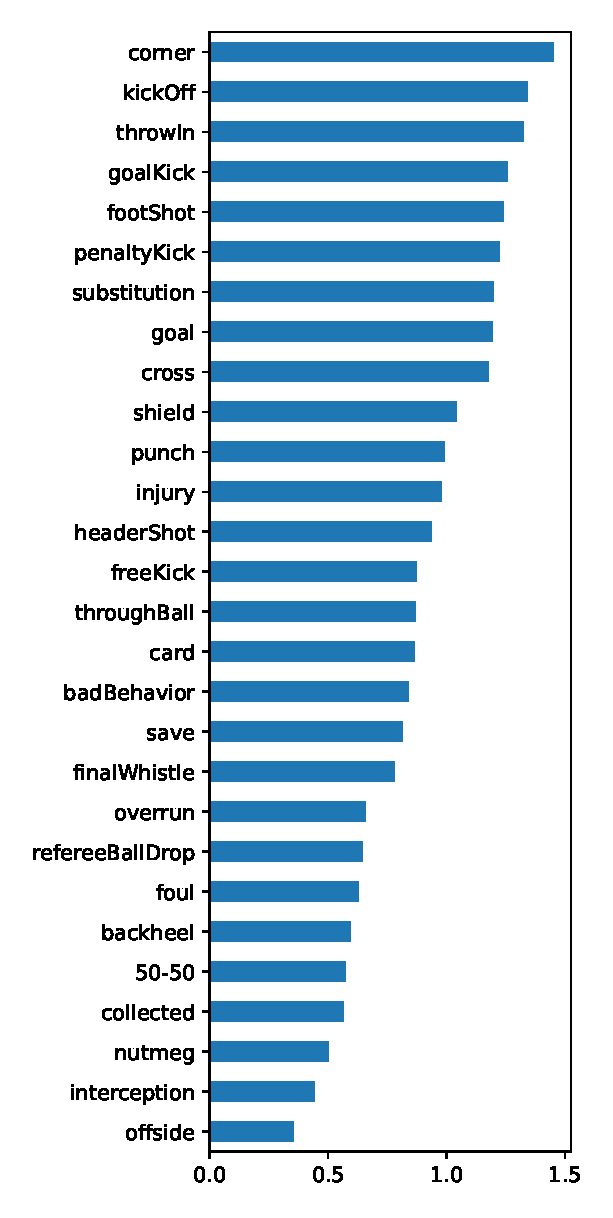
\includegraphics[width=0.99\textwidth, keepaspectratio, interpolate]{img/07_pca_by_class_socc_har_28.eps}
        \caption{PCA-0 \newline mit 28 Klassen}
    \end{subfigure}
    \begin{subfigure}{.24\textwidth}
        \centering
        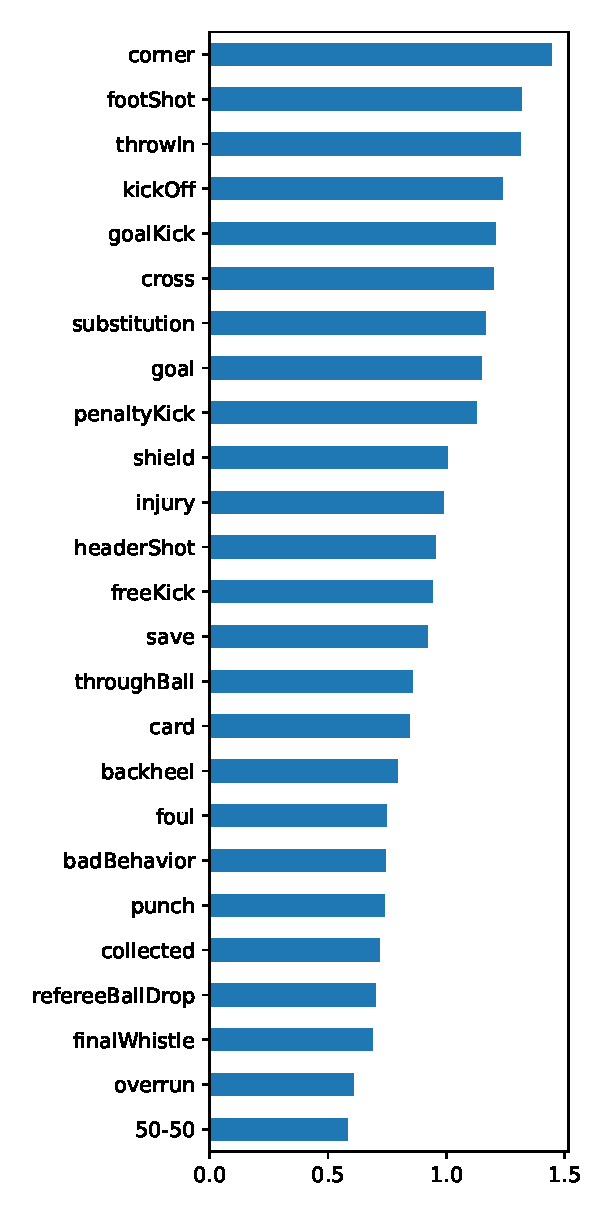
\includegraphics[width=0.99\textwidth, keepaspectratio, interpolate]{img/07_pca_by_class_socc_har_25.eps}
        \caption{PCA-0 \newline mit 25 Klassen}
        \label{fig:pca_by_class_phase_3}
    \end{subfigure}
    \caption[Vergleich der Aktionsklassen anhand erhobener Metriken]{Vergleich der Aktionsklassen anhand erhobener Metriken (Quelle: Eigene Darstellung)}
    \label{fig:class-metrics}
\end{figure}

%Dabei fällt auch auf, dass vor die Klassen im unteren Bereich mit einer niedrigen Precision viele False Positives verursachen, obwohl sie zum Teil einen hohen Recall haben.
%Auffällig ist auch, dass Aktionen, die sich im laufenden Spiel ereignen (\code{foul}, \code{cross}, \code{footShot}, \code{save}) einen besonders hohen Recall haben, während Aktionen die oft mit Spielunterbrechungen und Nahaufnahmen einhergehen (\code{substitution}, \code{goal}, \code{injury}) einen sehr niedrigen Recall aufweisen.

Da sich für jede erhobene Metrik eine abweichende Rangfolge der Klassen ergibt, ist es schwierig auf eine allgemeingültige Rangordnung zu schließen, die die Komplexität aller Klassen widerspiegelt.
Es kann also keine pauschale Aussage über die Komplexität einer Aktionsklasse gemacht werden.
Dennoch lässt sich anhand der erfassten Metriken eine grobe Ordnung erstellen, auch wenn sie allgemein nicht repräsentativ ist.
Hierzu werden alle fünf Metriken pro Klasse zu einer zweidimensionalen Matrix $M \in \mathbb{R}^{(\gls{tld:A} \times 5)}$ angeordnet und im Zuge einer \gls{pca} auf einen eindimensionalen Vektor projiziert.
Die erste Komponente der \gls{pca} $c_0 \in \mathbb{R}^{(5 \times 1)}$ deckt mit 80 \% hinreichend viel Varianz ab und projiziert die Metriken auf einen Vektor:

\begin{equation}
    \label{eq:pca}
    \text{pca}_0 = M \cdot c_0
\end{equation}

Die resultierende Rangordnung ist in \autoref{fig:pca_by_class_phase_2} abgebildet.
Als Folge werden die schwächsten vier Klassen aus dem ursprünglichen Datenset entfernt und das Modell wird erneut mit den übrigen 28 Klassen und $\Theta_\text{train} = 300$ nachtrainiert.
Anschließend wird dieser Prozess erneut wiederholt, indem drei weitere Klassen entfernt werden und das Modell nur mit den 25 besten Klassen nachtrainier wird.
Nach beiden Trainings wurden wieder jeweils 50 Samples verifiziert und dabei insgesamt 187 weitere Transaktionen vorgenommen, um die Datenqualität zu verbessern.

Durch das Ausschließen dieser besonders schweren Klassen konnte eine zusätzliche Steigerung der Balanced Accuracy von 2.4~\% \bzw 6.4~\% erwirkt werden.
Das Modell mit 25 Klassen gilt fortan als Baseline-Modell der dritten Phase.
\autoref{fig:pca_by_class_phase_3} zeigt die dazu resultierende Ordnung der Klassen nach ihrer Schwierigkeit.
Analysiert man die Ordnung, fällt auf, dass vor allem Klassen, die einen hohen Detailgrad in der Erkennung erfordern (\code{nutmeg}, \code{handBall}, \code{deflected}) schlecht abschneiden.
Eine mögliche Erklärung ist die geringe Auflösung der Modelle, die nicht alle Informationen abbilden kann.
Das Gegenteil ist der Fall bei Klassen, die oft in Kombination mit Nahaufnahmen gezeigt werden, wie \code{injury} oder \code{substitution}.
Ebenfalls schlecht schneiden Klassen ab, die eine hohe Kontextabhängigkeit haben, wie \code{offside} oder \code{finalWhistle}.
Während Klassen, die durch räumliche Gegebenheiten (insbesondere der Spielfeldmarkierungen) geprägt sind (\code{kickOff}, \code{corner}, \code{throwIn}), deutlich besser abschneiden.

\section{Training mit erhöhter Auflösung}
\label{sec:fine-tuning}

\begin{tcolorbox}[title=WIP]
    \begin{itemize}
        \item Werte nachtragen
    \end{itemize}
\end{tcolorbox}

In der vierten Phase wird das Baseline-Modell der dritten Phase mit einer höheren Auflösung $S$ nachtrainiert.
Das Vorgehen, welches sich am in~\cite{Wu20} vorgestellten Multi-Grid-Training orientiert, erhöht die Auflösung alle 5 Epochen.
So wird ein zusätzliches Experiment mit $S=240$ und eins mit $S=256$ angesetzt.
Eine noch höhere Auflösung ist aufgrund der Hardware-Einschränkungen nicht möglich.
\autoref{tab:exp4} zeigt die Ergebnisse dieser und aller vorangegangenen Phase im Vergleich.

\begin{table}
    \centering
    \small
    \csvreader[no head,tabular=|l|l|r|r||r|r|r||r|r|r|,
    table head=\hline,late after line=\\\hline]{tbl/exp_phase_1-4.csv}
    {1=\phase,2=\s,3=\t,4=\lilTau,5=\bigDelta,6=\auroc,7=\ba,8=\fbeta,9=\bigTheta,10=\socchar}
    {\phase & \socchar & \bigTheta & \bigDelta & \s & \t & \lilTau & \ba & \fbeta & \auroc}
    \caption[Ergebnisse aus Phase 1 bis 4]{Ergebnisse aus Phase 1 bis 4\footnote{Ergebnisse und Beispiele online unter https://www.comet.ml/narendorf/socc-har-32-baselines}}
    \label{tab:exp4}
\end{table}

%\begin{figure}
%    \centering
%    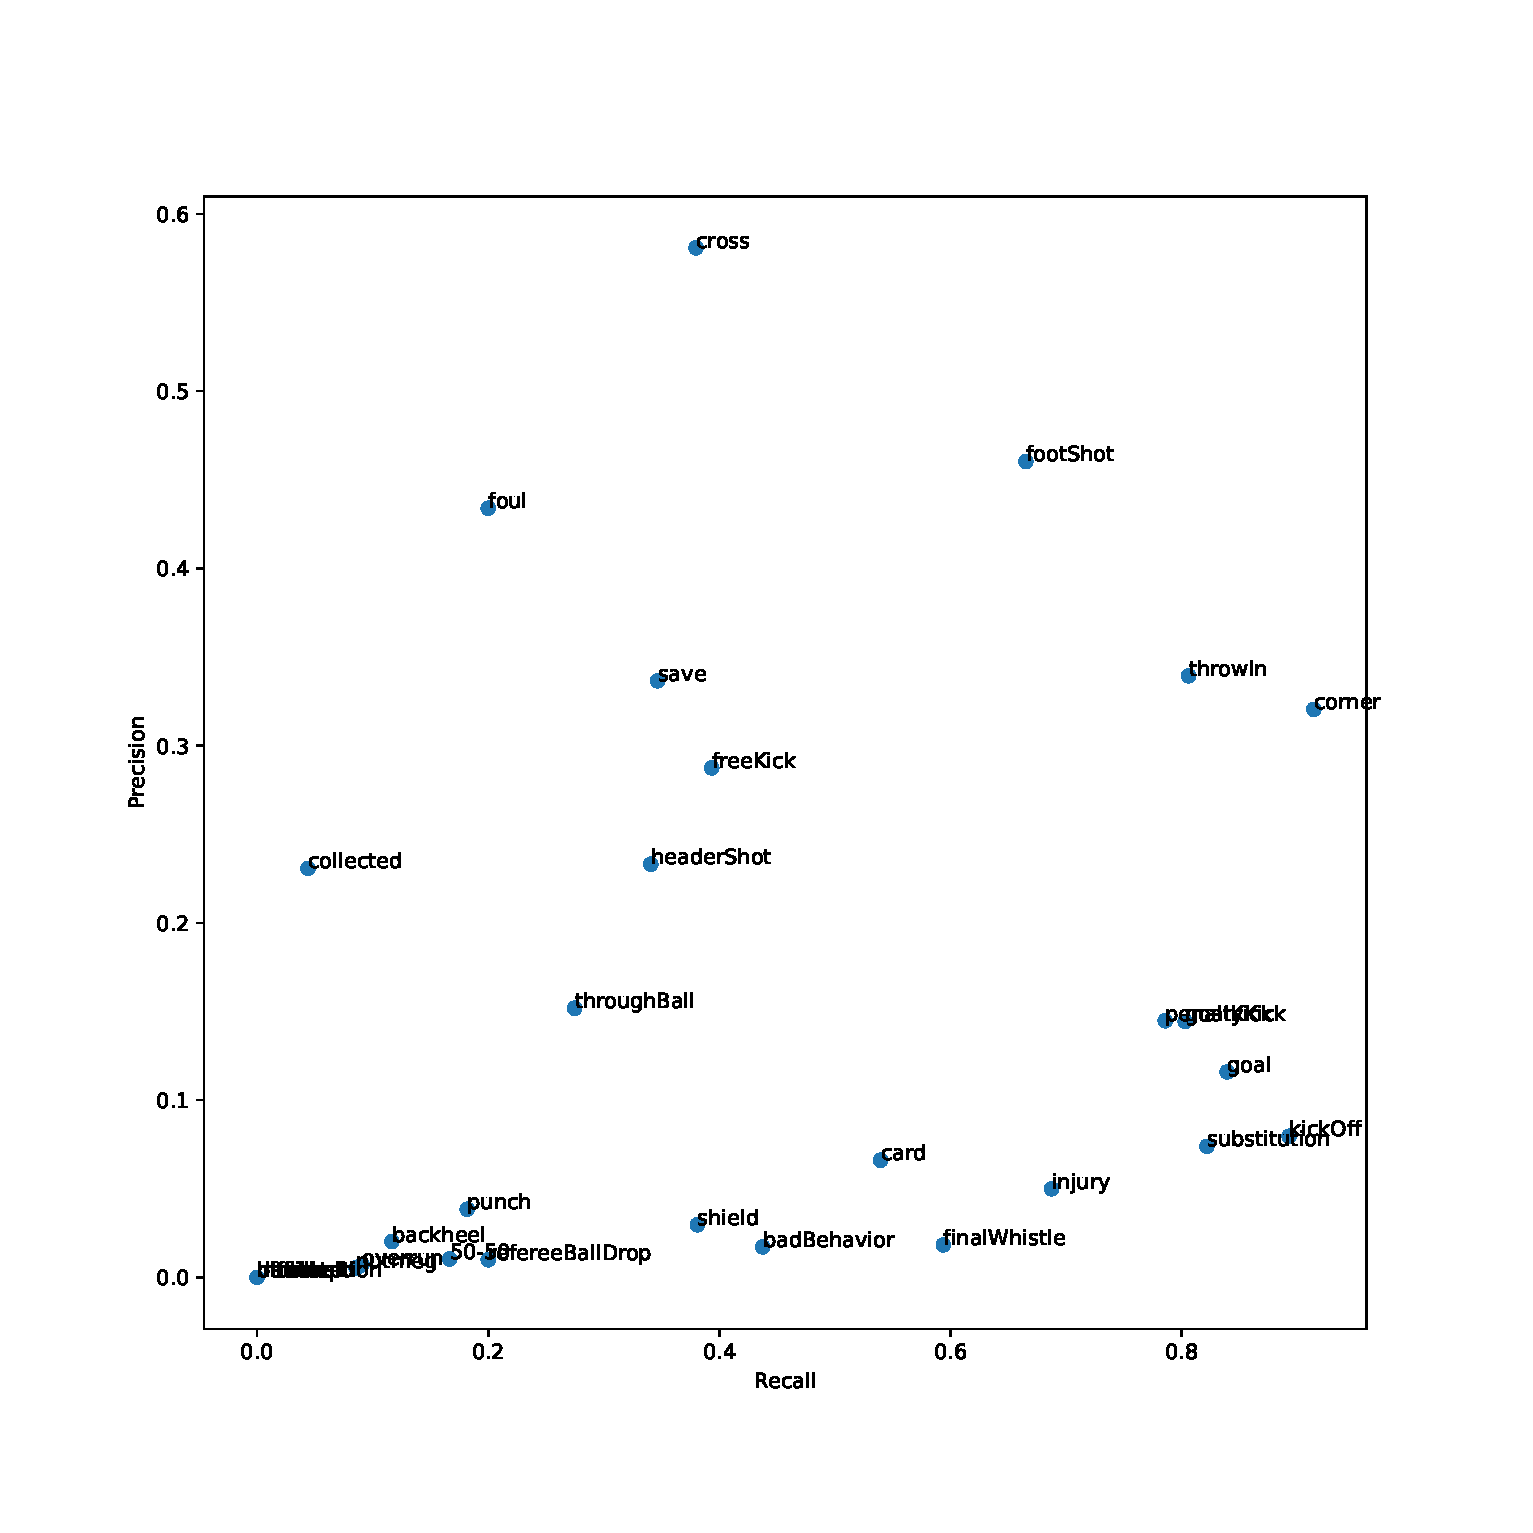
\includegraphics[width=0.99\textwidth, keepaspectratio, interpolate]{img/07_precision_recall_by_class.eps}
%    \caption{Vergleich von Precision und Recall pro Klasse}
%    \label{fig:precision-recall}
%\end{figure}

\section{Vergleich zu bestehenden Datensets}
\label{subsec:evaluation-auf-teilmengen}

Aufgrund des zeitlichen Rahmens dieser Arbeit war es nicht möglich einen direkten Vergleich des Baseline-Modells anhand der Original-Datensets von SoccerNet und SoccerDB durchzuführen.
Für eine grobe Einordnung wurden jedoch zwei weitere Untermengen von SOCC-HAR-32 abgeleitet -- mit den gleichen Aktionsklassen aus den genannten Datensets.
Das Baseline-Modell dieser Phase wurde anhand beider Subsets ohne weiteres Training evaluiert.
Die Ergebnisse in \autoref{tab:eval_subset} sind also keinesfalls direkt vergleichbar oder repräsentativ, da die Datengrundlage eine andere ist.
Es soll dem Leser jedoch eine grobe Einordnung ermöglichen.

\begin{table}
    \centering
    \small
    \csvreader[no head,tabular=|l||r|r|r|,
    table head=\hline,late after line=\\\hline]{tbl/eval_subsets.csv}
    {1=\dataset,2=\ba,3=\fbeta,4=\auroc}
    {\dataset & \ba & \fbeta & \auroc}
    \caption{Evaluation auf Teilmengen von Aktionsklassen}
    \label{tab:eval_subset}
\end{table}